\subsubsection{Q10.20 data 11092021 grouped by scenario}

\begin{comment}
               EFPR        EO      EFNR     n    pvalue
(frauth,)  0.477273  0.522727  0.477273  22.0  0.986772
(icu,)     0.500000  0.500000  0.647059  17.0  0.494974
(rent,)    0.416667  0.583333  0.444444  18.0  0.361935
\end{comment}

\begin{table}[h]
    \centering
    \begin{tabular}{|c|c|c|c|c|c|}
        \hline
        scenario & EFPR & EO & EFNR & n & p-value\\
        \hline
        frauth & 0.477 & \textbf{0.523} & 0.477 & 22.0 & 0.987\\
		icu & 0.500 & 0.500 & \textbf{0.647} & 17.0 & 0.495\\
		rent & 0.417 & \textbf{0.583} & 0.444 & 18.0 & 0.362\\
		
        \hline
    \end{tabular}
    \caption{Grouped by scenario}
    \label{tab:my_label}
\end{table}
\begin{figure}[h]
    \centering
    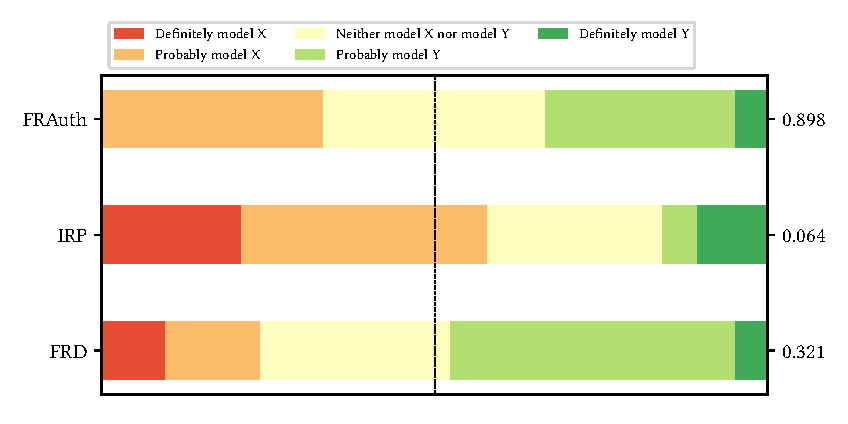
\includegraphics[width=0.8\textwidth]{figures/Q10.20/11092021/Q10.20_scenario.pdf}
    \caption{Grouped by scenario}
    \label{fig:my_label}
\end{figure}
